% =============================================================================
% §4 Design  — Route A: all five modules. Target: 2.5--2.8 pages.
% 4.5/5 bar: each module names the finding it answers; interfaces are concrete;
% what is forbidden is as clear as what is done.
% 填写: 换 Fig.~6--8；补 API 名字与真实阈值；不要新增第六个“也做了”的模块。
% =============================================================================
\section{Design}
\label{sec:design}

\sys{} is a userspace ANNS runtime plus a thin residency plane in front of host DRAM, a bounded window that plays the role of CXL-DRAM, and a flash-backed CXL address space that holds $D$ (Figure~\ref{fig:design-arch}).
Search is still best-first graph walk.
The service contract is a \emph{split}: prefetch and continuous batching may touch CXL-SSD; the scoring thread may not.
A hop that computes a full-precision distance from bytes that were not already in the window is a hide failure, not a successful promote.

The wise prefetcher turns a committed PQ rerank set into one precise page batch before full-precision scoring.
That precision does not remove the query's materialization barrier: its rerank still waits for its own batch.
Continuous batching exploits the independence across queries to cover that wait with other useful work.
The modules below separate these two roles and the evaluation tests them independently.

\begin{figure*}[t]
  \centering
  \phbox{0.98\textwidth}{3.8cm}{%
    Fig.~6 placeholder --- architecture:\\
    top: Placement $|$ Window admit $|$ Prefetch+\texttt{cont} $|$ $L$ ctrl;\\
    middle: residency plane (fill off crit path / score from window);\\
    bottom: host DRAM (graph/PQ) $|$ window $=$ virtual CXL-DRAM $|$ CXL-SSD.}
  \caption{\sys{} architecture.
    From the host, scored bytes look like CXL-DRAM; capacity is CXL-SSD.
    The residency plane is the only path that moves full-precision bytes.
    Search never page-faults a neighbor ``to be helpful.''
    \textbf{Fill-in:} use shipped names (\texttt{PREFETCH\_BATCH}, DramWindow); mark \texttt{vmem\_sw}.}
  \Description{Layered architecture of the ANNS runtime over three memory tiers.}
  \label{fig:design-arch}
\end{figure*}

\subsection{D1: Semantic placement}
\label{sec:d1}

Table~\ref{tab:placement} is the default map.
The graph adjacency and the PQ codebook are touched on every hop and are small relative to the full-precision corpus; they live in host DRAM so they never compete with vectors for the CXL-SSD window (F2, F7).
Query state (candidates, visited set, thread-local arenas) is likewise host-local.
Full-precision vectors default to the CXL-SSD address space.
A bounded \emph{hub / shared hot set} of vector pages is explicitly cached into the window or into CXL-DRAM (\S\ref{sec:d3}).
Only full-precision vectors in a committed rerank set become prefetch candidates; a discovered frontier does not (F3).

This is a deliberate difference from DiskANN, where adjacency and vectors share SSD sectors.
We pay a modest host-DRAM tax for the graph in order to stop the window from turning into an accidental adjacency cache.

\begin{table}[t]
  \caption{Default placement. \textbf{Fill-in:} bytes on the corpus you report (e.g., 25M $\times$ dim).}
  \label{tab:placement}
  \small
  \begin{tabular}{@{}p{0.28\columnwidth}p{0.22\columnwidth}p{0.42\columnwidth}@{}}
    \toprule
    Object & Default tier & Why \\
    \midrule
    Graph ($R$ neighbors) & host DRAM & every hop; keep off the window \\
    PQ / codebook        & host DRAM & tiny, extremely hot \\
    Query / visited      & host DRAM & per-worker state \\
    Full-precision vec.  & CXL-SSD   & capacity \\
    Entry / soft-pin     & window (tiny) & F7; LFU hot set demoted \\
    Committed rerank vec. & window via prefetch & F3, F5; score only if resident \\
    \bottomrule
  \end{tabular}
\end{table}

\subsection{D2: Wise prefetch at candidate commitment}
\label{sec:d2}

\paragraph{When: after commitment.}
The host first completes its approximate beam using the adjacency graph and PQ codes, without reading full-precision vectors from Flash.
When that beam commits the bounded rerank set $C_L$, the prefetcher issues immediately: after uncertainty has been pruned, but before exact scoring dereferences any vector in $C_L$.
This trigger deliberately gives up speculative lead time to avoid moving payload for candidates that will not survive.
The single-query path may still wait for materialization to complete; the invariant is that the subsequent scoring loads do not themselves fault on Flash.

\paragraph{What: the committed payload.}
The residency plane maps the IDs in $C_L$ to their full-precision vector pages, removes pages that are resident or already in flight, and deduplicates the rest.
Every requested page is therefore justified by at least one vector that exact reranking will consume.
Adjacency, PQ codes, speculative neighbors, and unused frontier records are not part of this wave.
Because Flash moves 4\,KiB pages, however, a justified page may still carry vector slots that this query will not score.

\paragraph{How: make each page useful.}
Offline, a co-use-aware layout groups vectors that disjoint training searches tend to request together and places the resulting pages into short runs.
Online, exact page filtering avoids duplicate movement, and the runtime fills gaps only in a short, sufficiently dense run; it never expands a sparse request into a whole SSD stripe.
This combination targets useful payload per read rather than batch size alone.
Unlike generic remote-memory or device-side sequential prefetchers~\cite{leap,cacheinhand}, the request is justified by the committed rerank set rather than an inferred address stream.
We distinguish page precision (a fetched page contains any scored vector), vector-slot utilization (scored slots over all slots read), and extent utilization (requested pages over pages transferred after coalescing); vector-slot utilization is the direct measure of real in-page use.

\begin{figure}[t]
  \centering
  \resizebox{0.88\columnwidth}{!}{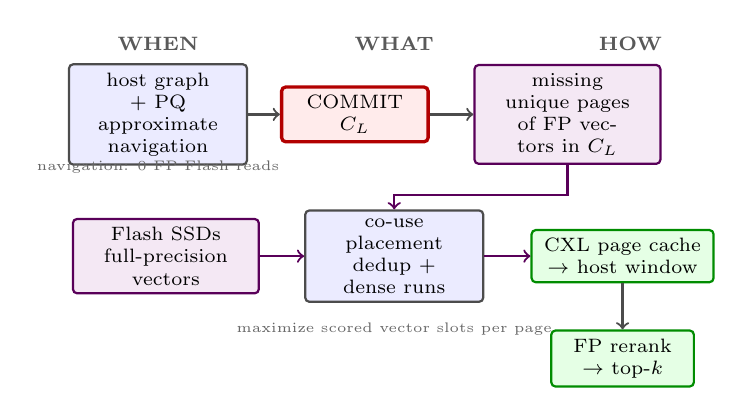
\begin{tikzpicture}[
  x=1cm,y=1cm,
  box/.style={draw=black!70, rounded corners=1.5pt, thick,
              align=center, inner sep=3pt, font=\scriptsize},
  info/.style={box, fill=blue!8},
  commit/.style={box, draw=red!70!black, fill=red!8, very thick},
  payload/.style={box, fill=violet!9, draw=violet!70!black},
  resident/.style={box, fill=green!10, draw=green!55!black},
  flow/.style={->, thick, draw=black!70},
  data/.style={->, thick, draw=violet!70!black},
  label/.style={font=\scriptsize\bfseries, text=black!65}
]
  \node[label] at (1.15,4.25) {WHEN};
  \node[label] at (4.15,4.25) {WHAT};
  \node[label] at (7.15,4.25) {HOW};

  \node[info,text width=2.05cm] (pq) at (1.15,3.35)
    {host graph + PQ\\approximate navigation};
  \node[commit,text width=1.65cm] (commit) at (3.65,3.35)
    {COMMIT\\$C_L$};
  \node[payload,text width=2.15cm] (select) at (6.35,3.35)
    {missing unique pages\\of FP vectors in $C_L$};
  \draw[flow] (pq)--(commit);
  \draw[flow] (commit)--(select);
  \node[font=\tiny,text=black!60,align=center] at (1.15,2.68)
    {navigation: 0 FP Flash reads};

  \node[payload,text width=2.15cm] (flash) at (1.25,1.55)
    {Flash SSDs\\full-precision vectors};
  \node[info,text width=2.05cm] (shape) at (4.15,1.55)
    {co-use placement\\dedup + dense runs};
  \node[resident,text width=2.10cm] (window) at (7.05,1.55)
    {CXL page cache\\$\rightarrow$ host window};
  \node[resident,text width=1.60cm] (rerank) at (7.05,0.25)
    {FP rerank\\$\rightarrow$ top-$k$};

  \draw[data] (select.south) -- ++(0,-0.38) -| (shape.north);
  \draw[data] (flash)--(shape);
  \draw[data] (shape)--(window);
  \draw[flow] (window)--(rerank);

  \node[font=\tiny,text=black!60,align=center] at (4.15,0.62)
    {maximize scored vector slots per page};
\end{tikzpicture}
}
  \caption{Wise prefetch answers three questions.
    \emph{When}: after PQ navigation commits $C_L$.
    \emph{What}: only missing unique pages of its full-precision vectors.
    \emph{How}: co-use-aware placement, exact filtering, and dense short runs increase useful vector slots per Flash read.}
  \Description{A left-to-right pipeline showing PQ candidate commitment, selection of missing full-precision vector pages, locality-aware request formation, materialization into the CXL cache and host window, and exact reranking.}
  \label{fig:design-promote}
\end{figure}

\subsection{D3: Entry pin and soft-pin (hot set demoted)}
\label{sec:d3}

Single-query deepening is a bad way to spend a small window (F4, F7).
A 64\,MiB shared LFU set raised hit rate and \emph{destroyed} QPS on a warm protocol (14.3$\rightarrow$2.4); we do not ship it as D3.
What remains is a tiny hard pin of the entry subgraph ($\le$32\,MiB) and a hop-decaying soft-pin of recently installed pages.
Pinning is never implicit in a page fault.
Cross-query reuse, if it happens, is because committed materialization left useful pages in the window---not because an LFU daemon is competing with search.

\subsection{D4: Hide engine --- wise prefetch and continuous batching}
\label{sec:d4}

\paragraph{A query-local barrier.}
D2 creates one precise materialization wave after PQ navigation commits $C_L$,
but the same query cannot rerank until that wave completes.
Better page selection alone therefore cannot keep Flash busy.

\paragraph{Cross-query overlap.}
The barrier is local to a query, not to the service: while one query waits,
another can navigate, materialize its own committed wave, or rerank resident
bytes.
Continuous batching interleaves these stages so host work and Flash access
coexist (Figure~\ref{fig:design-pipe}).
Like continuous scheduling in other staged serving systems~\cite{orca}, it
admits work at a semantic boundary---candidate commitment rather than a model
iteration.

\paragraph{Bounded admission.}
The runtime bounds in-flight query stages and admits another committed wave as
capacity becomes available, avoiding both device bubbles and an unbounded work
queue.
It neither predicts future candidates nor implements adaptive queue-depth
control.

\paragraph{Semantic invariance.}
Each query retains the same graph, PQ codes, beam budget, and visited state, and
reranks only after its own pages are resident.
Batching changes timing, but not its candidate set or recall.

\begin{figure*}[t]
  \centering
  \resizebox{0.98\textwidth}{!}{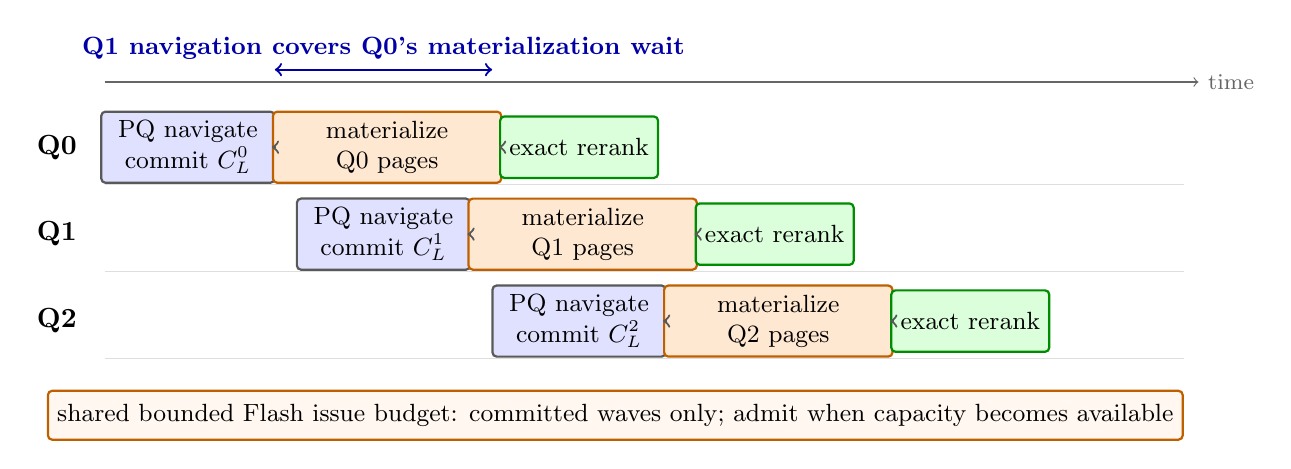
\begin{tikzpicture}[
  x=0.92cm,y=0.92cm,
  font=\small,
  lane/.style={font=\bfseries,anchor=east},
  stage/.style={draw=black!65,thick,rounded corners=1.5pt,
                minimum height=0.78cm,align=center,font=\small},
  nav/.style={stage,fill=blue!12},
  materialize/.style={stage,fill=orange!18,draw=orange!75!black},
  rank/.style={stage,fill=green!14,draw=green!55!black},
  flow/.style={->,thick,draw=black!65}
]
  \draw[->,black!60] (1.20,4.95)--(16.30,4.95)
    node[anchor=west,font=\footnotesize] {time};
  \node[font=\small\bfseries,blue!65!black] at (5.05,5.42)
    {Q1 navigation covers Q0's materialization wait};
  \draw[<->,thick,blue!65!black] (3.55,5.12)--(6.55,5.12);

  \node[lane] at (0.95,4.05) {Q0};
  \node[lane] at (0.95,2.85) {Q1};
  \node[lane] at (0.95,1.65) {Q2};
  \foreach \y in {4.05,2.85,1.65}
    \draw[black!13] (1.20,\y-0.52)--(16.10,\y-0.52);

  \node[nav,minimum width=2.20cm] (q0n) at (2.35,4.05)
    {PQ navigate\\commit $C_L^0$};
  \node[materialize,minimum width=2.90cm] (q0m) at (5.10,4.05)
    {materialize\\Q0 pages};
  \node[rank,minimum width=2.00cm] (q0r) at (7.75,4.05)
    {exact rerank};
  \draw[flow] (q0n)--(q0m); \draw[flow] (q0m)--(q0r);

  \node[nav,minimum width=2.20cm] (q1n) at (5.05,2.85)
    {PQ navigate\\commit $C_L^1$};
  \node[materialize,minimum width=2.90cm] (q1m) at (7.80,2.85)
    {materialize\\Q1 pages};
  \node[rank,minimum width=2.00cm] (q1r) at (10.45,2.85)
    {exact rerank};
  \draw[flow] (q1n)--(q1m); \draw[flow] (q1m)--(q1r);

  \node[nav,minimum width=2.20cm] (q2n) at (7.75,1.65)
    {PQ navigate\\commit $C_L^2$};
  \node[materialize,minimum width=2.90cm] (q2m) at (10.50,1.65)
    {materialize\\Q2 pages};
  \node[rank,minimum width=2.00cm] (q2r) at (13.15,1.65)
    {exact rerank};
  \draw[flow] (q2n)--(q2m); \draw[flow] (q2m)--(q2r);

  \node[draw=orange!75!black,thick,rounded corners=1.5pt,fill=orange!6,
        minimum width=11.9cm,minimum height=0.62cm,font=\small]
    at (8.25,0.35)
    {shared bounded Flash issue budget: committed waves only; admit when capacity becomes available};
\end{tikzpicture}
}
  \caption{Continuous batching fills the service-level bubbles left by a
    single precise materialization wave.
    When Q0 waits for its committed pages, Q1 and Q2 contribute navigation,
    Flash materialization, or reranking under a bounded in-flight budget.
    Each query still crosses its own materialization barrier before reranking,
    so scheduling changes timing but not search semantics.}
  \Description{Three query timelines overlap host-side PQ navigation,
    bounded asynchronous Flash materialization, and exact reranking.  Each
    query reranks only after its own committed pages become resident.}
  \label{fig:design-pipe}
\end{figure*}

\subsection{D5: Observability}
\label{sec:d5}

Every experiment in~\S\ref{sec:eval} is required to report hide counters first: fraction of full-precision scores whose bytes were already in the window (\texttt{score\_from\_window}), critical-path NAND wait (\texttt{crit\_wait\_ns}), and device-fill/wall overlap, then QPS at the iso-recall floor.
Prefetch efficiency is reported as page precision, vector-slot utilization, and extent utilization; a page touched once is not evidence that all of its payload was useful.
QPS without those counters is not a hide result.

\paragraph{What we refuse to hide.}
If a module cannot move \texttt{crit\_wait\_ns} or \texttt{score\_from\_window} in an ablation, it is removed from the contribution list rather than kept as decoration.
An LFU hot set that raises hit rate and drops QPS is already in that bin.
